% LaTeX file for resume 
% This file uses the resume document class (res.cls)

\documentclass{res} 
%\usepackage{helvetica} % uses helvetica postscript font (download helvetica.sty)
%\usepackage{newcent}   % uses new century schoolbook postscript font 
\newsectionwidth{0pt}  % So the text is not indented under section headings
\usepackage{fancyhdr}  % use this package to get a 2 line header
\usepackage{hyperref}  % use this package to provide url links
%\usepackage{mdwlist}	% use this package for customizing lists
\usepackage{graphicx}
\renewcommand{\headrulewidth}{0pt} % suppress line drawn by default by fancyhdr
\setlength{\headheight}{24pt} % allow room for 2-line header
\setlength{\headsep}{24pt}  % space between header and text
\setlength{\headheight}{24pt} % allow room for 2-line header
\pagestyle{fancy}     % set pagestyle for document
\rhead{ {\it K. Apicharttrisorn's Resume}\hspace{0.2in}{\it p. \thepage} } % put text in header (right side)
\cfoot{}                                     % the foot is empty
\topmargin=-0.5in % start text higher on the page

\begin{document}
\thispagestyle{empty} % this page has no header  
\name{KITTIPAT APICHARTTRISORN\\[12pt]}% the \\[12pt] adds a blank line after name
\hfill 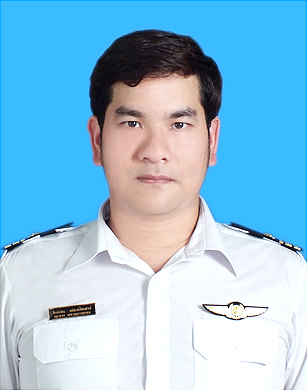
\includegraphics[scale=1]{myphoto2}
\address{{\bf Office Address} \\ Air Traffic Data Systems Engineering Department \\
  Aeronautical Radio of Thailand \\   Sathon, Bangkok, Thailand 10120 \\ (+66) 2285-9177}    
                                      
\address{{\bf Permanent Address} \\ 7/639 Vibhavadee-Rangsit Rd. \\ Chatuchak, Bangkok 10900\\
  (+66) 2537-0097}



\begin{resume}
 
\section{\centerline{OBJECTIVE}}
\vspace{6pt} % provide vertical space between section title and contents
A Ph.D. student position in computer science with research interest in computer networks, distributed resource allocation, sensor networks, software-defined networking, and internet of things. 
 
\vspace{0.05in}
\section{\centerline{EDUCATION}} 
\vspace{6pt} 
{\sl Master of Science}, Computer Science \\
Chulalongkorn University, Bangkok, Thailand \hspace{0.2in}  GPA 3.75 / 4.00 \hfill May 2007 - November 2010 \\
THESIS - Distributed Time Synchronization in Wireless Sensor Networks \\
ADVISOR - Asst. Prof. Dr. Chalermek Intanagonwiwat
 
{\sl Bachelor of Engineering}, Electrical Engineering \\ % \sl will be bold italic in
					 % New Century Schoolbook (or
					 % any postscript font) and
					 % just slanted in Computer
					 % Modern (default) font
Kasetsart University, Bangkok, Thailand  \hspace{0.2in}  GPA 2.49 / 4.00    \hfill    June 2000 - October 2004 \\
SENIOR PROJECT: Adaptive Multi-Rate - Wideband (AMR-WB) speech codec Testing\\
SENIOR PROJECT SUPERVISOR: Assoc. Prof. Dr. Mongkol Raksapatcharawong\\

\vspace{0.05in} 
\section{\centerline{EMPLOYMENT}} 
\vspace{6pt}
{\sl Senior Systems Engineer} \hfill        January 2007 - Present \\
Air Traffic Data Systems Engineering Department \\
  Aeronautical Radio of Thailand, Bangkok, Thailand       
  
\begin{itemize} \itemsep -2pt % reduce space between items
   \item Administer, monitor, and maintain aeronautical data systems for which the Air Traffic Data Systems Engineering Department take responsibility so that the systems operate to support availability, safety and continuity of air navigation services
   \item Perform preventive maintenance, corrective maintenance, software and hardware installation, and deployment of monitoring systems (e.g. ICMP, SNMP)
   \item Inspect and troubleshoot problems, coordinate and consult with related internal and external aeronautical units to troubleshoot problems and investigate causes of interruption or outage of data systems services
   \item Gather information from users and report usage and service problems to managers, programmers and the director, to improve systems' reliability, availability and serviceability
 \end{itemize}
 
{\sl Network Engineer} \hfill                  March 2005 - September 2006 \\
1tonet Co., Ltd., Bangkok, Thailand
  \begin{itemize} \itemsep -2pt
  \item Design and implement voice over IP subsystems
 \item  Integrate IP telephony with customers' existing public exchange systems
 %\item  Test and report IP telephone call quality, e.g. voice clarity and delay, to the technical manager
 \end{itemize}
 \newpage
\section{\centerline{PUBLICATIONS}} 
\vspace{18pt}
\begin{itemize}
%	\item \textbf{``A Stable and Equitable Desynchronization Algorithm for Multi-Hop Wireless Sensor Networks''}
%		\begin{description}\itemsep -2pt 
%		\item[Authors]Supasate Choochaisri, Kittipat Apicharttrisorn and Chalermek Intanagonwiwat
%		\item[Publication Name]ACM Transactions on Sensor Networks (TOSN)
%		\item[Publication Date]\textit{Under submission}
%		\item[Abstract]{\sl \small  N/A }
%		\end{description}
%	\vspace{2pt}
	\item \textbf{``A Moving Object Tracking Algorithm Using Support Vector Machines in Binary Sensor Networks''}
		\begin{description}\itemsep -2pt 
		\item[Authors]Dusadee Apicharttrisorn, Kittipat Apicharttrisorn and Teerasit Kasetkasem
		\item[Publication Name]The 13th International Symposium on Communications and Information Technologies
		\item[Publication Date]September 2013
		\item[Abstract]{\sl \small Wireless sensor technologies have enabled us to deploy such small sensors to monitor an area of interest. Object tracking is one of the most attractive applications to be implemented with wireless sensor networks (WSNs). However, many solutions are struggled with energy-draining global positioning system (GPS), poorly-performed trilateration for indoor usage, and impractical, complex algorithms to be implemented in sensor nodes. This paper proposes a moving object tracking algorithm using support vector machines (MOT-SVM). The MOT-SVM takes advantage of light-weighted directional binary sensor networks, and state-of-the-art signal processing algorithms, namely the support vector machines and particle filters. We compare our proposed algorithm with the Aslam's work through the simulation. We examine our algorithms for various movement scenarios such as the linear, random and the 8-model trajectories, and the scenarios in which observing sensors make observation errors.}
		\end{description}
   \vspace{2pt}
	\item \textbf{``Desynchronization with an artificial force field for wireless networks''}
		\begin{description}\itemsep -2pt 
		\item[Authors]Supasate Choochaisri, Kittipat Apicharttrisorn, Kittiporn Korprasertthaworn, Pongpakdi Taechalertpaisarn and  Chalermek Intanagonwiwat
		\item[Publication Name]SIGCOMM Computer Communication Review
		\item[Publication Date]March 2012 
		\item[Abstract]{\sl \small Desynchronization is useful for scheduling nodes to perform tasks at different time. This property is desirable for resource sharing, TDMA scheduling, and collision avoiding. Inspired by robotic circular formation, we propose DWARF (Desynchronization With an ARtificial Force field), a novel technique for desynchronization in wireless networks. Each neighboring node has artificial forces to repel other nodes to perform tasks at different time phases. Nodes with closer time phases have stronger forces to repel each other in the time domain. Each node adjusts its time phase proportionally to its received forces. Once the received forces are balanced, nodes are desynchronized. We evaluate our implementation of DWARF on TOSSIM, a simulator for wireless sensor networks. The simulation results indicate that DWARF incurs significantly lower desynchronization error and scales much better than existing approaches.}
		\end{description}
 	\vspace{2pt}
	\item \textbf{``Energy-Efficient Gradient Time Synchronization for Wireless Sensor Networks''}
		\begin{description}\itemsep -2pt 
		\item[Authors]Kittipat Apicharttrisorn, Supasate Choochaisri and Chalermek Intanagonwiwat
		\item[Publication Name]2010 Second International Conference on Computational Intelligence, Communication Systems and Networks (CICSyN)
		\item[Publication Date]July 2010
		\item[Abstract]{\sl \small Wireless sensor network (WSN) applications usually demand a time-synchronization protocol for node coordination and data interpretation. In this paper, we propose an Energy-Efficient Gradient Time Synchronization Protocol (EGTSP) for Wireless Sensor Networks. In contrast to FTSP, a state-of-the-art synchronization protocol for WSNs, EGTSP is a completely localized algorithm that achieves a global time consensus and gradient time property using effective drift compensation and incremental averaging estimation. In contrast with GTSP, a gradient-based fixed-rated time synchronization protocol, our protocol provides adaptive beaconing for applications to optimize energy savings by selecting appropriate message-broadcast periods. The protocol is implemented and evaluated on multi-hop networks that consist of Telosb motes running TinyOS. The experimental results indicate that our protocol achieves a network-wide global notion of time, attains small synchronization errors, and utilizes energy efficiently.}
		\end{description}
  \end{itemize}
\newpage
\section{\centerline{ACADEMIC PROJECTS}} 
\vspace{18pt}
	\begin{itemize} 
		\item Project Name: Time Synchronization for Wireless Sensor Networks
			\begin{description} \itemsep -2pt 
			\item[Objective] MS Thesis's Research Project 
			\item[Description]Time synchronization is a challenging but important task for wireless sensor networks (WSNs) because of the resource-constrained characteristics. This project aims to explore a distributed protocol and algorithm of time synchronization that is time-accurate and energy-efficient while maintaining a gradient time property.
			\item[Period] January 2008 - October 2010
			\item[Roles and Responsibility]	Main investigator who reviews literature, designs, analyzes, and implements algorithms, finally produces a publication			
			\item[Tools and Environments] TinyOS, Ubuntu, Gnuplot, TelosB* motes
			\end{description}		
		\item Project Name: Desynchronization as Distributed Resource Allocations and TDMA
			\begin{description} \itemsep -2pt
				\item[Objective] Research Project 
				\item[Description] Desynchronization is an abstraction that arranges nodes declaring to access a shared resource in a round-robin schedule. It can be applied to solve resource allocation problems especially in distributed systems. This research project aims to explore a novel distributed desynchronization algorithm.
				\item[Period] March 2010 - Present
				\item[Roles and Responsibility]	Literature review, experiments, and publications			
				\item[Tools and Environments]TinyOS, TOSSIM, Ubuntu, Gnuplot
			\end{description}
		\item Project Name: Moving Object Tracking in Binary Sensor Networks
			\begin{description} \itemsep -2pt
				\item[Objective] Research Project
				\item[Description] Moving object tracking is a potential application of wireless sensor networks. Binary sensor networks require nodes only to send one-bit information to the central processing node which is responsible for signal processing tasks to track a moving object. This research project aims to explore a signal processing algorithm that tracks the object more accurately with tolerance to signal errors.
				\item[Period] March 2013 - Present
				\item[Roles and Responsibility]	Literature review, experiments, and publications			
				\item[Tools and Environments] Matlab
			\end{description}		
		\item Project Name: Distributed Online Ticket Reservation with Display on Google Maps
			\begin{description} \itemsep -2pt
				\item[Objective] Term Project (Graduate Course: Distributed Systems)
				\item[Description] This project aims to provide an opportunity for students to design and implement a distributed system which reserves online tickets and displays the status through Google Maps.
				\item[Period] June 2008 - October 2008
				\item[Roles and Responsibility]	Design overall systems and demonstration			
				\item[Tools and Environments] Microsoft .NET and Google Map APIs
			\end{description}							
		\item Project Name: Thailand's Undergrad Admission Systems: Information Systems Architecture
			\begin{description} \itemsep -2pt
				\item[Objective] Term Project (Graduate Course: Information Systems Architecture)
				\item[Description]This project aims to provide an opportunity for students to design Thailand's Undergrad Admission Systems. During this term project, we  combine each other's experience and viewpoints of information systems and brainstorm the viable solutions for the systems.  The final document consists of the design of network, database, hardware, middleware, and software. The designed architecture is supposed to support thousands of concurrent users who use the system from registrations to final admission reports.
				\item[Period] June 2007 - October 2007
				\item[Roles and Responsibility]	Part of group discussion and brainstroming sessions		
				\item[Tools and Environments] MS Words, MS Visio
			\end{description}
			\newpage
		\item Project Name: Adaptive Multi-Rate - Wideband (AMR-WB) speech codec Testing
			\begin{description} \itemsep -2pt
				\item[Objective] Undergraduate Senior Project (Electrical Engineering Project)
				\item[Description] Adaptive Multi-Rate Wideband (AMR-WB) is a patented wideband speech coding standard developed based on Adaptive Multi-Rate encoding, using similar methodology as Algebraic Code Excited Linear Prediction (ACELP). AMR-WB provides improved speech quality due to a wider speech bandwidth of 50 - 7000 Hz compared to narrowband speech coders which in general are optimized for POTS wireline quality of 300 - 3400 Hz. This project aims to document the study of AMR-WB in both theoretical and practical aspects.
				\item[Period] June 2003 - Mar 2004
				\item[Roles and Responsibility]	Design and conduct experiments, and document a project report 			
				\item[Tools and Environments] MS Visual C
			\end{description}	
	\end{itemize}
* TelosB is a WSN platform that is widely used by research laboratories worldwide.	
\vspace{0.1in} 
\section{\centerline{PROFESSIONAL PROJECTS}} 
\vspace{15pt}
\begin{itemize} \itemsep -2pt
		\item Project Name: Aeronautical Message Switching Systems (AMSS)
		\begin{description} \itemsep -2pt 
			\item[Description] AMSS is a core aeronautical data system that switches, stores and manipulates aeronautical messages interexchanged between aeronautical units worldwide so that flights are operated and managed properly and continuously.
			\item[Roles and Responsibilities]Administer, monitor, and maintain the system, inspect and troubleshoot problems
			\item[Tools and Environments] Redhat Enterprise, Windows Servers, Oracle Database 10g, Cisco switches and routers 
		\end{description}
		\item Project Name: Aeronautical Message Handling Systems (AMHS) and X.400
		\begin{description} \itemsep -2pt 
			\item[Description] According to ICAO*, Aeronautical Message Handling System is a new standard for aeronautical ground-ground communications (e.g. for the transmission of NOTAM**, Flight Plans or Meteorological Data) based on X.400 profiles. Aeronautical Radio of Thailand progresses to establish AMHS connectivity with several countries such as India, Singapore, Hong Kong, Italy, Laos, Vietnam, and Cambodia.
			\item[Roles and Responsibilities]Test and record system connectivity and functionality
			\item[Tools and Environments] Redhat Enterprise, Oracle Database 10g, ATN Routers
		\end{description}
		\item Project Name: Flight Data Management Center
		\begin{description} \itemsep -2pt 
			\item[Description] Flight Data Management Center was established to unify clearance of national flight plans and their modifications to a single center in order to streamline air navigation operations. Computer-based systems are used to provide the functionality of FDMC.
			\item[Roles and Responsibilities]Administer, monitor, and maintain the system, inspect and troubleshoot problems
			\item[Tools and Environments] Java, Redhat Enterprise, MS Windows Servers, Oracle Database, Cisco switches and routers 
		\end{description}
		\item Project Name: Operational Aeronautical Meteorological Data (OPMET) and Regional OPMET Bulletins Exchange (ROBEX) Systems
		\begin{description} \itemsep -2pt 
			\item[Description] Aeronautical Radio of Thailand was designated to provide a regional OPMET data bank of the Asia/Pacific region. Its core function is to accumulate and store aeronautical meteorological data that can be retrieved remotely and automatically by queries from relevant aeronautical organizations. ROBEX processes such data in the form of bulletins, a periodic conclusive report,  and periodically send them to related aeronautical units.
			\item[Roles and Responsibilities]Administer, monitor, and maintain the systems, inspect and troubleshoot problems
			\item[Tools and Environments] Java, Redhat Enterprise, MS Windows Servers, Oracle Database, Cisco switches and routers 
		\end{description}
\end{itemize}
\vspace{-2pt}
* ICAO (International Civil Aviation Organization) is a specialized agency of the United Nations which codifies the principles and techniques of international air navigation and fosters the planning and development of international air transport to ensure safe and orderly growth. Its headquarters are located in the Quartier International of Montreal, Quebec, Canada.

** NOTAM (Notice to Airmen) is a notice filed with an aviation authority to alert aircraft pilots of potential hazards along a flight route or at a location that could affect the safety of the flight. Aeronautical Radio of Thailand is authorized to provide a NOTAM data bank that stores and retrieves NOTAM messages which are distributed by AMSS and AMHS.
\vspace{0.1in} 
\section{\centerline{GRANTS}} 
\vspace{12pt}
 \begin{itemize} \itemsep -2pt 
	\item Grant Name: International Conference Attendance Support Grants for Graduate Students
		\indent \begin{description} \itemsep -2pt \topsep 0pt
			\item[Period] July 2010
			\item[Purpose] This grant provides partial financial support for graduate students whose academic papers are accepted to be presented at an international conference.
			\item[Amount] Approximately 900 USD 
			\item[Granted by] Graduate School, Chulalongkorn University Bangkok, Thailand
		\end{description}
	\item Grant Name: AINTEC* 2010 Conference Attendance Grants
		\begin{description} \itemsep -2pt 
			\item[Period] November 2010
			\item[Purpose] This grant provides full financial support for graduate students who are interested in Internet research so that they can attend and participate in this academic conference.
			\item[Amount] Attendance Fee (Unknown) 
			\item[Granted by]  Thailand Research Education Network Association (ThaiREN), Bangkok, Thailand
		\end{description}
	\item Grant Name: AINTEC* 2008 Conference Attendance Grants
		\begin{description} \itemsep -2pt 
			\item[Period] November 2008
			\item[Purpose]This grant provides full financial support for graduate students who are interested in Internet research so that they can attend and participate in this academic conference.
			\item[Amount] Attendance Fee (Unknown) 
			\item[Granted by]  Thailand Research Education Network Association (ThaiREN), Bangkok, Thailand
		\end{description}
\end{itemize} 
\vspace{-5pt}
* AINTEC (Asian INTernet Engineering Conference) is an international conference held in Thailand and hosted by Internet Education and Research Laboratory, Asian Institute of Technology, Thailand \url{http://www.interlab.ait.ac.th/}. This single-tracked conference attracts high-quality papers from global Internet research communities.
 
\vspace{0.2in} 
\section{\centerline{ACADEMIC ACTIVITIES}} 
\vspace{18pt}
\begin{itemize}
	\item \begin{description}
		\item[Event] IEEE International Conference on Computer Communications (INFOCOM 2012) 
		\item[Activity] Review papers delegated by Asst. Prof. Dr. Chalermek Intanagonwiwat
	\end{description} 
	\item \begin{description}
		\item[Event] IEEE International Conference on Computer Communications (INFOCOM 2011) 
		\item[Activity] Review papers delegated by Asst. Prof. Dr. Chalermek Intanagonwiwat
	\end{description} 
\end{itemize}

\vspace{0.2in} 
 \section{\centerline{ CERTIFICATES }}
 \vspace{18pt} 
\begin{itemize}
\item Certificate Name: \textit{``Embedded Software Engineering''}  
	\begin{description}
 		\item[Content] Embedded Hardware Architecture, Operating Systems for Embedded Systems, Programming Embedded Systems, Embedded Systems I/O, Embedded Software Engineering
 		\item[Certified by] Computer Engineering Department, Chulalongkorn University and Software Industry Promotion Agency (SIPA)
 		\item[Duration] 22 - 27 October 2007
 	\end{description}  
\item Certificate Name: \textit{``Certified Thaicom Users''} 
	\begin{description}
 		\item[Content] General functionality of THAICOM satellites, Basic VSAT setup, Signal optimization and interference
 		\item[Certified by] THAICOM Public Company Limited
 		\item[Duration] 3 April 2007
 	\end{description} 
\item Certificate Name: \textit{``Network Design and Implementation I''} 
 	\begin{description}
 		\item[Content] Design, analysis, implementation and troubleshooting of computer networks and hands-on workshops with CISCO routers and switches
 		\item[Certified by] Continuing Education Center, Chulalongkorn University
 		\item[Duration] 29 January 2005 - 23 April 2005
 	\end{description}
\end{itemize}
\vspace{0.1in} 
\section{\centerline{ SKILLS }}
\vspace{8pt} 
\normalsize{\section{Programming Languages}}
                 \begin{itemize}
                 \item C, C++, NesC, TinyOS, Matlab, Java, Python, SQL
                 \end{itemize}
\normalsize{\section{Computer Software}} 
                 \begin{itemize}
                  \item Ubuntu, UNIX, Gnuplot, Latex. 
                  \end{itemize}
\normalsize{\section{Language Proficiency}}
	           \begin{itemize} 
                   \item English: TOEFL 107 iBT  (Test Date: 24 November 2013) \\ Reading: 26 / 30, Listening: 29 / 30, Speaking: 22 / 30, Writing: 30 / 30
                  \item Thai: Native 
                   \end{itemize}
\normalsize{\section{Graduate Record Examination}}
	           \begin{itemize} 
                   \item Test Date: 21 October 2013
                  \item Verbal Reasoning Score: 152 / 170 (\textit{$53^{rd}$ Percentile Rank})
                  \item Quantitative Reasoning Score: 164 / 170 (\textit{$89^{th}$ Percentile Rank})
                  \item Analytical Writing Score: 4.0 / 6.0 (\textit{$54^{th}$ Percentile Rank})
                   \end{itemize}
\vspace{0.1in}                   
\section{\centerline{VOLUNTEER SERVICES}} 
\vspace{15pt}
\begin{itemize}
\item Event Name: CANSO* Global ATM Summit and 15th Annual General Meeting (AGM)
\begin{description} \itemsep -2pt 
\item[Period] 11 June 2011 - 14 June 2011
\item[Description]: As Air Chief Marshal Somchai Thean-anant, a former President of Aeronautical Radio of Thailand delivered a policy to recruit the company's employees to volunteer to help organize these eminent events that welcomed hundreds of worldwide dignitaries and executives from all segments of the aviation industry.  I applied for a volunteer position and  was then selected, under the supervision of Ms. Tipaporn Nippakakorn, Vice President (Human Resource), to help organize the conference and seminar rooms at the Renaissance Hotel, Bangkok.
\item[Contributions]: Help organize meeting rooms
\item[Benefits]: Overall, the company succeeded in organizing these meetings which brought about and strengthen collaboration and understanding between global aeronautical organizations. My personal benefits included friendship with other employees from various departments of the company and awareness of aviation industry's next generation gathered during the conference and seminar attendance. Most importantly, I learn to volunteer myself to contributing back to my organization and aviation society without any pay.
\end{description}
*CANSO – the Civil Air Navigation Services Organization – is the global voice of air navigation service providers (ANSPs) worldwide. CANSO's members support over 85 percent of world air traffic and share information and develop new policies, with the ultimate aim of improving air navigation services (ANS) on the ground and in the air.
\end{itemize}
\vspace{0.1cm}
\section{\centerline{INTERESTS AND HOBBIES}} 
\vspace{-2pt} 
\begin{center}
Jazz and blues guitar, photography,  cooking, swimming
\end{center} 
%\newpage
\section{\centerline{REFERENCES}} 
\vspace{18pt}
		\begin{itemize}
		\item Ms. Tipaporn Nippakakorn
		\begin{description}\itemsep -2pt 
			\item[Position] Vice President (Human Resource)
			\item[Address] Aeronautical Radio of Thailand, Bangkok, Thailand, 10120
			\item[Email] tipaporn.ni@aerothai.co.th
			\item[Tel.] (+66) 2285-9179
		\end{description}
		\item Dr. Chalermek Intanagonwiwat
		\begin{description}\itemsep -2pt 
			\item[Position] Senior Software Engineer
			\item[Address] Cisco Systems, Inc., California, USA
			\item[Email] cintanag@cisco.com
			\item[Tel.] (+1) 408 525 3795
		\end{description}				
		\item Mr. Pongnarin Anantasirijinda
			\begin{description}\itemsep -2pt 
				\item[Position]Director of Air Traffic Data Systems Engineering Department
				\item[Address]Aeronautical Radio of Thailand, Bangkok, Thailand, 10120
				\item[Email]add@aerothai.co.th
				\item[Tel.](+66) 2285-9101
			\end{description}		        
		\item Asst. Prof. Dr. Teerasit Kasetkasem
			\begin{description}\itemsep -2pt 
				\item[Position]Assistant Professor of Electrical Engineering
				\item[Address]Electrical Engineering Department, Kasetsart University, Bangkok, Thailand, 10900
				\item[Email]fengtsk@ku.ac.th
				\item[Tel.](+66) 2942-8555 ext 1536
			\end{description}
		 %\item Dr. Supasate Choochaisri
		% 	\begin{description}\itemsep -2pt 
%		 		\item[Position]Co-founder and Operations Manager
%		 		\item[Address]Larngear Technology Co., Ltd., Software Park Bld. Nonthaburi, Thailand 11120
%		 		\item[Email] supasate.c@gmail.com
%		 		\item[Tel.](+66) 2584-6064
%		 	\end{description}
		\end{itemize}


 
\end{resume}

\end{document}













